\documentclass[12pt,a4paper]{article}

% ─── Page Layout ───────────────────────────────────────────────────────────────
\usepackage[a4paper, margin=0.8in, headheight=14pt]{geometry}

% ─── Fonts (XeLaTeX) ───────────────────────────────────────────────────────────
\usepackage{fontspec}
\usepackage{unicode-math}
\setmainfont{TeX Gyre Pagella}
\setmonofont[Scale=0.88]{TeX Gyre Cursor}
\setmathfont{Latin Modern Math}

% ─── Packages ──────────────────────────────────────────────────────────────────
\usepackage{xcolor}
\usepackage{colortbl}
\usepackage{titlesec}
\usepackage{enumitem}
\usepackage{tabularx}
\usepackage{booktabs}
\usepackage{array}
\usepackage{amsmath}
\usepackage{tikz}
\usetikzlibrary{shapes.geometric, arrows.meta, positioning, calc, fit, decorations.pathreplacing}
\usepackage{tcolorbox}
\tcbuselibrary{skins, breakable}
\usepackage{hyperref}
\usepackage{fancyhdr}
\usepackage{graphicx}
\usepackage{microtype}
\hyphenpenalty=10000
\exhyphenpenalty=10000
\sloppy
\usepackage{caption}
\usepackage{setspace}
\usepackage{multirow}
\usepackage{tocloft}

% ─── Q&A helper ────────────────────────────────────────────────────────────────
\newcommand{\Q}[1]{\textbf{#1}\par\noindent\ignorespaces}

% ─── Colour Palette ────────────────────────────────────────────────────────────
\definecolor{myred}{RGB}{196,30,58}
\definecolor{mydark}{RGB}{30,30,50}
\definecolor{mygreen}{RGB}{14,120,80}
\definecolor{myteal}{RGB}{0,130,140}
\definecolor{myamber}{RGB}{180,100,0}
\definecolor{mypurple}{RGB}{100,30,160}
\definecolor{mygray}{RGB}{246,247,249}
\definecolor{mgframe}{RGB}{180,185,200}
\definecolor{watermark}{RGB}{145,150,170}
\definecolor{hdrred}{RGB}{250,232,235}
\definecolor{hdrgreen}{RGB}{220,244,233}
\definecolor{hdrteal}{RGB}{220,242,244}
\definecolor{hdramber}{RGB}{253,242,215}
\definecolor{hdrpurple}{RGB}{238,228,255}
\definecolor{hdrgray}{RGB}{238,240,245}
\definecolor{rowalt}{RGB}{250,251,253}

% ─── Section Formatting ────────────────────────────────────────────────────────
\titleformat{\section}
  {\large\bfseries\color{myred}}{\thesection.}{0.5em}{}
  [\vspace{1pt}{\color{myred}\rule{\linewidth}{0.8pt}}]
\titleformat{\subsection}
  {\normalsize\bfseries\color{myteal}}{\thesubsection}{0.5em}{}
\titlespacing*{\section}{0pt}{18pt}{7pt}
\titlespacing*{\subsection}{0pt}{11pt}{4pt}

% ─── Paragraph ─────────────────────────────────────────────────────────────────
\setlength{\parindent}{0pt}
\setlength{\parskip}{4pt}

% ─── TOC Styling ───────────────────────────────────────────────────────────────
\renewcommand{\cfttoctitlefont}{\large\bfseries\color{myred}}
\renewcommand{\cftaftertoctitle}{\par\noindent{\color{myred}\rule{\linewidth}{0.8pt}}}
\setlength{\cftbeforetoctitleskip}{0pt}
\setlength{\cftaftertoctitleskip}{6pt}
\renewcommand{\cftsecfont}{\normalsize\bfseries\color{mydark}}
\renewcommand{\cftsecpagefont}{\normalsize\bfseries\color{mydark}}
\renewcommand{\cftsecleader}{\cftdotfill{\cftdotsep}}
\setlength{\cftbeforesecskip}{7pt}
\renewcommand{\cftsubsecfont}{\small\color{mydark}}
\renewcommand{\cftsubsecpagefont}{\small\color{mydark}}
\setlength{\cftbeforesubsecskip}{3pt}
\setlength{\cftsubsecindent}{1.4em}

% ─── Table helpers ─────────────────────────────────────────────────────────────
\renewcommand{\arraystretch}{1.45}
\setlength{\tabcolsep}{6pt}
\arrayrulecolor{mydark}
\newcolumntype{B}[1]{>{\small\bfseries\raggedright\arraybackslash}m{#1}}
\newcolumntype{Y}{>{\small\raggedright\arraybackslash}X}
\renewcommand{\tabularxcolumn}[1]{m{#1}}

% ─── Header / Footer ───────────────────────────────────────────────────────────
\pagestyle{fancy}
\fancyhf{}
\fancyhead[L]{\small\color{myred}\textbf{PE-EC801A}\;\color{mydark}--- Antennas and Propagation}
\fancyhead[R]{\small\color{myteal}\textbf{Module 6 Notes}}
\fancyfoot[C]{\small\color{mydark}\thepage}
\fancyfoot[R]{\small\color{watermark}\textit{\copyright\ Biraj}}
\renewcommand{\headrulewidth}{0.5pt}
\renewcommand{\footrulewidth}{0.3pt}

% ─── Hyperref ──────────────────────────────────────────────────────────────────
\hypersetup{
  colorlinks=true, linkcolor=myteal, urlcolor=myteal,
  pdfauthor={Biraj Sarkar},
  pdftitle={PE-EC801A --- Module 6 Notes}
}

% ─── tcolorbox styles ──────────────────────────────────────────────────────────
\tcbset{
  tikzbox/.style={
    colback=mygray, colframe=mgframe, boxrule=0.6pt, arc=4pt,
    left=8pt, right=8pt, top=6pt, bottom=6pt,
    colbacktitle=mgframe, coltitle=mydark,
    fonttitle=\small\bfseries
  },
  defbox/.style={
    colback=hdrgreen, colframe=mygreen, boxrule=0.8pt, arc=4pt,
    left=9pt, right=9pt, top=6pt, bottom=6pt,
    colbacktitle=mygreen, coltitle=white,
    fonttitle=\small\bfseries
  },
  formulabox/.style={
    colback=hdrteal, colframe=myteal, boxrule=0.8pt, arc=4pt,
    left=9pt, right=9pt, top=7pt, bottom=7pt,
    colbacktitle=myteal, coltitle=white,
    fonttitle=\small\bfseries
  },
  examplebox/.style={
    colback=hdramber, colframe=myamber, boxrule=0.8pt, arc=4pt,
    left=9pt, right=9pt, top=6pt, bottom=6pt,
    colbacktitle=myamber, coltitle=white,
    fonttitle=\small\bfseries
  },
  masonbox/.style={
    colback=hdrpurple, colframe=mypurple, boxrule=0.8pt, arc=4pt,
    left=9pt, right=9pt, top=6pt, bottom=6pt,
    colbacktitle=mypurple, coltitle=white,
    fonttitle=\small\bfseries
  },
  exambox/.style={
    colback=hdrpurple, colframe=mypurple, boxrule=1pt, arc=5pt,
    left=10pt, right=10pt, top=8pt, bottom=8pt,
    colbacktitle=mypurple, coltitle=white,
    fonttitle=\bfseries,
    breakable, title after break={\textbf{Frequently Asked / Viva Questions (contd.)}}}
}
\tcbset{breakable}

% ─── TikZ styles ───────────────────────────────────────────────────────────────
\tikzset{
  block/.style={rectangle, draw=myteal, fill=hdrteal,
    text width=2.4cm, align=center, minimum height=0.95cm,
    font=\small, rounded corners=3pt, line width=0.7pt},
  redblock/.style={rectangle, draw=myred, fill=hdrred,
    text width=2.4cm, align=center, minimum height=0.95cm,
    font=\small, rounded corners=3pt, line width=0.7pt},
  netnode/.style={rectangle, draw=myteal, fill=hdrteal,
    text width=1.5cm, align=center, minimum height=0.8cm,
    font=\small, rounded corners=3pt, line width=0.7pt},
  sumjunc/.style={circle, draw=myamber, fill=hdramber,
    minimum size=0.62cm, font=\small, line width=0.8pt},
  snode/.style={circle, draw=mypurple, fill=hdrpurple,
    minimum size=0.55cm, font=\footnotesize, line width=0.7pt},
  arrow/.style={-Stealth, thick, color=mydark},
  redarrow/.style={-Stealth, thick, color=myred},
  line/.style={thick, color=mydark}
}

% ═══════════════════════════════════════════════════════════════════════════════
\begin{document}
% ═══════════════════════════════════════════════════════════════════════════════

\begin{center}
  {\LARGE\bfseries\color{myred} PE-EC801A --- Antennas and Propagation}\\[5pt]
  {\normalsize\color{mydark} Semester VIII \quad$\bullet$\quad 3L:0T:0P \quad$\bullet$\quad 3 Credits}\\[3pt]
  {\normalsize\color{myteal}\textbf{Module 6 Exam Notes}}\\[3pt]
  {\small\color{mydark} CGEC \;$|$\; B.Tech ECE (2023--27) \;$|$\; \textit{Biraj Sarkar}}
\end{center}
\vspace{2pt}
\noindent{\color{myred}\rule{\linewidth}{1.5pt}}
\vspace{2pt}

\hypersetup{linkcolor=mydark}
\tableofcontents
\hypersetup{linkcolor=myteal}
\newpage

% ===============================================================================
\section{Uniform Linear Arrays (ULA)}
% ===============================================================================

\begin{tcolorbox}[defbox, title={\textbf{Definition of an Antenna Array}}]
An \textbf{antenna array} is a set of two or more identical antenna elements positioned and excited such that their individual radiation fields combine constructively in desired directions and cancel destructively in other directions, increasing directivity.
\end{tcolorbox}

\subsection{Two-Element Array Analysis}
Consider two identical antennas separated by a distance $d$ along the $z$-axis. Antenna 1 is at the origin and serves as the phase reference ($I_1 = I_0 e^{j0}$). Antenna 2 is fed with a phase lead $\beta$ ($I_2 = I_0 e^{j\beta}$).

\begin{tcolorbox}[tikzbox, title={Two-Element Array Geometry}]
\centering
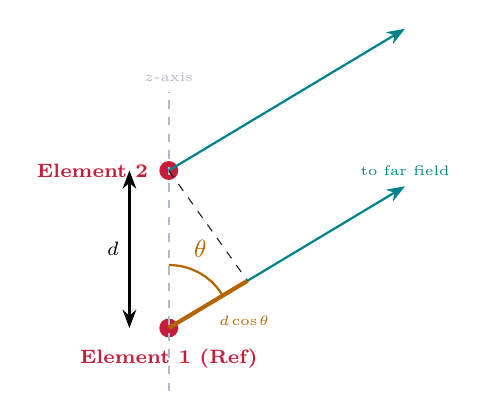
\begin{tikzpicture}[scale=1.0]
  % Antennas
  \fill[myred] (0,0) circle (0.12) node[below=4pt, font=\scriptsize\bfseries] {Element 1 (Ref)};
  \fill[myred] (0,2.0) circle (0.12) node[left=4pt, font=\scriptsize\bfseries] {Element 2};

  % Array axis
  \draw[dashed, thick, color=mgframe] (0,-0.8) -- (0,3.0) node[above, font=\tiny] {$z$-axis};

  % Rays to far field
  \draw[-Stealth, thick, color=myteal] (0,0) -- (3.0,1.8) node[above, font=\tiny] {to far field};
  \draw[-Stealth, thick, color=myteal] (0,2.0) -- (3.0,3.8);

  % Perpendicular for path difference
  \draw[dashed, color=mydark] (0,2.0) -- (1.0, 0.6);
  \draw[line width=1.5pt, color=myamber] (0,0) -- (1.0,0.6) node[midway, below right, font=\tiny\bfseries] {$d\cos\theta$};

  % Angle
  \draw[thick, color=myamber] (0,0.8) arc (90:31:0.8);
  \node[color=myamber, font=\small\bfseries] at (0.4, 1.0) {$\theta$};

  % Spacing
  \draw[Stealth-Stealth, thick] (-0.5,0) -- (-0.5,2.0) node[midway, left, font=\scriptsize] {$d$};

\end{tikzpicture}
\end{tcolorbox}

In the far field, the path difference between the waves is $d\cos\theta$ (where $\theta$ is measured from the array axis). The total phase difference $\psi$ between the fields is:
\[
\psi = kd\cos\theta + \beta
\]
The total far-field electric field is:
\[
E_{total} = E_1 + E_2 = E_0 \left( 1 + e^{j(kd\cos\theta + \beta)} \right) = E_0 e^{j\psi/2} \left( 2\cos\frac{\psi}{2} \right)
\]
The normalized \textbf{Array Factor (AF)} is:
\[
AF_n(\theta) = \cos\left( \frac{kd\cos\theta + \beta}{2} \right)
\]

\subsection{N-Element Uniform Linear Array (ULA)}
For $N$ identical elements fed with equal amplitude $I_0$ and progressive phase shift $\beta$:
\[
AF = \sum_{n=0}^{N-1} e^{j n (kd\cos\theta + \beta)} = \sum_{n=0}^{N-1} e^{j n \psi}
\]
Summing this geometric progression:
\[
|AF| = \left| \frac{\sin\left(\frac{N}{2}\psi\right)}{\sin\left(\frac{1}{2}\psi\right)} \right| \implies |AF_n| = \left| \frac{\sin\left(\frac{N}{2}(kd\cos\theta + \beta)\right)}{N \sin\left(\frac{1}{2}(kd\cos\theta + \beta)\right)} \right|
\]

\subsection{Broadside vs. End-Fire Arrays}
\begin{enumerate}[label=\textbf{\arabic*.}, leftmargin=*, itemsep=4pt]
  \item \textbf{Broadside Array:} Maximum radiation is perpendicular to the array axis ($\theta = 90^\circ$).
    \begin{itemize}[leftmargin=*, itemsep=1pt]
      \item \textit{Condition:} $\psi = 0$ at $\theta = 90^\circ \implies kd\cos(90^\circ) + \beta = 0 \implies \beta = 0$.
      \item \textit{Nulls:} Occur when $\sin(N\psi/2) = 0 \implies \theta_{null} = \cos^{-1}\left( \pm \frac{m\lambda}{Nd} \right), \quad m = 1, 2, 3, \dots$
    \end{itemize}
  \item \textbf{End-Fire Array:} Maximum radiation is along the array axis ($\theta = 0^\circ$ or $180^\circ$).
    \begin{itemize}[leftmargin=*, itemsep=1pt]
      \item \textit{Condition for $\theta = 0^\circ$:} $\psi = 0 \implies kd\cos(0^\circ) + \beta = 0 \implies \beta = -kd$.
      \item \textit{Condition for $\theta = 180^\circ$:} $\psi = 0 \implies kd\cos(180^\circ) + \beta = 0 \implies \beta = kd$.
    \end{itemize}
\end{enumerate}

% ===============================================================================
\section{Non-Uniform Amplitude Arrays}
% ===============================================================================

Uniform arrays have high directivity but suffer from relatively high sidelobes ($-13.5\,\text{dB}$ for the first sidelobe). To reduce sidelobes, elements can be excited with non-uniform current amplitudes.

\subsection{Binomial Array}
The excitation amplitudes of the elements correspond to the coefficients of a binomial expansion:
\[
a_n = \binom{N-1}{n}, \quad n = 0, 1, \dots, N-1
\]
For example, for a 5-element array, the amplitudes scale as $1 : 4 : 6 : 4 : 1$.
\begin{itemize}[leftmargin=*, itemsep=2pt]
  \item \textbf{Advantage:} Completely eliminates sidelobes if the element spacing $d \le \lambda/2$.
  \item \textbf{Disadvantage:} Broader beamwidth (HPBW) and lower directivity than a uniform array of equivalent length.
\end{itemize}

\subsection{Dolph-Tschebyscheff Array}
This array uses Tschebyscheff (Chebyshev) polynomials $T_m(z)$ to design a pattern with a specified sidelobe level (SLL) and the narrowest possible main beamwidth.
The Chebyshev polynomials are defined by:
\[
T_m(z) = \cos(m \cos^{-1} z) \quad (|z| \le 1)
\]
\[
T_m(z) = \cosh(m \cosh^{-1} z) \quad (|z| > 1)
\]
This method optimizes the trade-off by ensuring that all sidelobes are at the exact same specified level (e.g., $-20\,\text{dB}$ or $-30\,\text{dB}$).

\textbf{Design Procedure:}
\begin{enumerate}[label=\textbf{\arabic*.}, leftmargin=*, itemsep=3pt]
  \item Specify the number of elements $N$ (array order $m = N-1$) and the desired sidelobe level ratio $R$ (e.g., $R = 26.3$ for $-20\,\text{dB}$ SLL; $R = 10^{SLL_{dB}/20}$).
  \item Compute the parameter $z_0$ that maps the main lobe maximum to $T_m(z_0)$:
  \[
  z_0 = \cosh\!\left[ \frac{1}{m} \cosh^{-1}(R) \right]
  \]
  \item Substitute $z = z_0 \cos\!\left(\frac{\psi}{2}\right)$ into $T_m(z)$ to obtain the array polynomial. The AF takes the form $AF(\psi) = T_m\!\left(z_0 \cos\frac{\psi}{2}\right)$.
  \item Extract the excitation coefficients $a_n$ by expanding the Chebyshev polynomial in powers of $\cos^n\!\left(\frac{\psi}{2}\right)$.
\end{enumerate}

\textbf{Key result:} For a 5-element array with $-20\,\text{dB}$ SLL, the excitation amplitudes are approximately $1 : 2.41 : 3.14 : 2.41 : 1$ (compare to binomial $1:4:6:4:1$ — Dolph gives a narrower beam for the same SLL).

% ===============================================================================
\section{Extension to Planar Arrays}
% ===============================================================================

A \textbf{planar array} consists of elements positioned in a two-dimensional grid (e.g., $M$ elements along $x$ with spacing $d_x$, and $N$ elements along $y$ with spacing $d_y$).

The overall Array Factor is the product of the individual linear array factors along the two directions:
\[
AF_{planar} = AF_x \cdot AF_y = \left[ \frac{\sin\left(\frac{M}{2}\psi_x\right)}{\sin\left(\frac{1}{2}\psi_x\right)} \right] \left[ \frac{\sin\left(\frac{N}{2}\psi_y\right)}{\sin\left(\frac{1}{2}\psi_y\right)} \right]
\]
where:
\[
\psi_x = k d_x \sin\theta \cos\phi + \beta_x
\]
\[
\psi_y = k d_y \sin\theta \sin\phi + \beta_y
\]
By dynamically adjusting the phase shifters $\beta_x$ and $\beta_y$, the main beam can be steered to any coordinate ($\theta_0, \phi_0$) in 3D space:
\[
\beta_x = -k d_x \sin\theta_0 \cos\phi_0
\]
\[
\beta_y = -k d_y \sin\theta_0 \sin\phi_0
\]

% ===============================================================================
\section{Antenna Array Synthesis}
% ===============================================================================

Array synthesis involves finding the feeding currents (amplitudes and phases) and element locations required to produce a desired radiation pattern.

\subsection{Schelkunoff Polynomial Method}
Schelkunoff represented the array factor of an $N$-element linear array as a polynomial in the complex variable $z = e^{j\psi}$:
\[
AF = \sum_{n=0}^{N-1} a_n z^n = a_{N-1} (z - z_1)(z - z_2) \dots (z - z_{N-1})
\]
where $z_i$ are the roots (zeros) of the polynomial. Since $z$ lies on the unit circle ($|z| = 1$), the nulls in the radiation pattern correspond to the roots that lie on the unit circle.

\textbf{Visible Region:} As $\theta$ varies from $0^\circ$ to $180^\circ$, $\psi = kd\cos\theta + \beta$ traces an arc on the unit circle in the complex $z$-plane. This arc is called the \textbf{visible region}:
\[
-kd + \beta \le \psi \le kd + \beta
\]
\begin{itemize}[leftmargin=*, itemsep=3pt]
  \item For $d = \lambda/2$ and $\beta = 0$: visible region spans $-\pi \le \psi \le \pi$ (full circle).
  \item For $d < \lambda/2$: visible region is less than a full circle — some roots in the \textbf{invisible region} do not contribute to the radiation pattern.
  \item Placing a root \textit{inside} the visible region creates a null in the pattern. Placing a root \textit{outside} the visible region eliminates that null.
\end{itemize}
This allows designers to synthesize specific patterns by precisely controlling which roots lie on vs. off the visible arc.

\subsection{Woodward-Lawson Method}
The Woodward-Lawson method synthesizes a desired source pattern by superimposing several independent, orthogonal beams (each having a $\frac{\sin(N\psi/2)}{N\sin(\psi/2)}$ shape centred at different angles). The excitation coefficients are found by sampling the desired pattern at the beam centres.

\textbf{Sampling formula:} For $N$ elements, the array factor is:
\[
AF(\psi) = \sum_{m=-(N-1)/2}^{(N-1)/2} c_m \cdot \frac{\sin\!\left[\frac{N}{2}(\psi - \psi_m)\right]}{N\sin\!\left[\frac{1}{2}(\psi - \psi_m)\right]}
\]
where each beam is centred at $\psi_m = \frac{2\pi m}{N}$ and the sampling coefficients $c_m$ are found by evaluating the desired pattern $F_d(\psi)$ at those points:
\[
c_m = F_d(\psi_m) = F_d\!\left(\frac{2\pi m}{N}\right)
\]

\textbf{Key properties:}
\begin{itemize}[leftmargin=*, itemsep=2pt]
  \item The synthesized pattern passes exactly through the desired sample values.
  \item Between sample points, the approximation may deviate (Gibbs-like ripple for abrupt transitions).
  \item Adding more elements $N$ increases the number of sample points and improves accuracy.
  \item Suitable for pencil-beam, sector, flat-top, or shaped beam synthesis.
\end{itemize}

% ===============================================================================
% MANDATORY QUICK REVISION PAGE
% ===============================================================================
\newpage
\begin{center}
  {\large\bfseries\color{myred} Quick Revision --- Module 6}\\[3pt]
  {\small\color{mydark} Antenna Arrays and Synthesis $|$ PE-EC801A}
\end{center}
\noindent{\color{myred}\rule{\linewidth}{1.2pt}}
\vspace{4pt}

\begin{tcolorbox}[formulabox, title={\textbf{Key Formulas and Metrics at a Glance}}]
\renewcommand{\arraystretch}{1.35}
\begin{tabularx}{\linewidth}{B{5.2cm} X}
N-Element ULA Array Factor ($AF$) & $AF = \frac{\sin(N\psi/2)}{\sin(\psi/2)}$ \quad where $\psi = kd\cos\theta + \beta$ \\[4pt]
Broadside Phase Shift ($\beta$) & $\beta = 0$ \\[4pt]
End-Fire Phase Shift ($\beta$) & $\beta = \mp kd$ \quad (for $\theta = 0^\circ$ or $180^\circ$ main beam) \\[4pt]
Binomial Array Coefficients & $a_n = \binom{N-1}{n} = \frac{(N-1)!}{n!(N-1-n)!}$ \\[4pt]
Planar Beam Steering Phase & $\beta_x = -k d_x \sin\theta_0 \cos\phi_0, \quad \beta_y = -k d_y \sin\theta_0 \sin\phi_0$ \\[4pt]
Schelkunoff Complex Variable ($z$) & $z = e^{j\psi} = e^{j(kd\cos\theta + \beta)}$ \\
\end{tabularx}
\end{tcolorbox}

\begin{tcolorbox}[defbox, title={\textbf{One-Line Definitions}}]
\begin{itemize}[leftmargin=*, itemsep=2pt, topsep=0pt]
  \item \textbf{Array Factor:} The radiation pattern of an array of isotropic elements, describing how the geometry and feeds affect the pattern.
  \item \textbf{Grating Lobe:} An unwanted duplicate main beam of radiation that occurs when element spacing $d \ge \lambda$.
  \item \textbf{Binomial Array:} An array with non-uniform excitation coefficients that completely eliminates sidelobes.
  \item \textbf{Phased Array:} An array where the phase of each element is dynamically adjusted to steer the radiation beam without moving the antenna.
  \item \textbf{Woodward-Lawson Method:} A pattern synthesis technique based on the superposition of orthogonal beam patterns.
\end{itemize}
\end{tcolorbox}

\begin{tcolorbox}[exambox, title={\textbf{Frequently Asked / Viva Questions}}]
\begin{enumerate}[topsep=0pt, label=\textbf{Q\arabic*.}, itemsep=5pt]
  \item \Q{Define Array Factor ($AF$). State the Principle of Pattern Multiplication.}
    The Array Factor is the radiation pattern of the array assuming isotropic radiating elements. The Principle of Pattern Multiplication states that the total far-field pattern ($E_{total}$) of an array of identical non-isotropic elements is the product of the single-element field pattern ($E_{single}$) and the Array Factor ($AF$):
    \[
    E_{total}(\theta, \phi) = E_{single}(\theta, \phi) \times AF(\theta, \phi)
    \]
  \item \Q{Differentiate between broadside and end-fire arrays.}
    A broadside array radiates its maximum power perpendicular to the axis of the array ($\theta = 90^\circ$), which requires in-phase feeds ($\beta = 0$). An end-fire array radiates along the axis ($\theta = 0^\circ$ or $180^\circ$), which requires a progressive phase shift $\beta = \mp kd$.
  \item \Q{What are grating lobes? How can they be avoided in array design?}
    Grating lobes are secondary maximum beams that have the same amplitude as the main beam. They represent a waste of energy in undesired directions. They can be avoided by keeping the element spacing smaller than a wavelength ($d < \lambda$, or $d < \lambda/2$ for steering).
  \item \Q{Why are binomial arrays designed? What is their main drawback?}
    Binomial arrays are designed to completely eliminate sidelobes in their radiation pattern. Their main drawback is that they produce a wider main beam width (reduced resolution) and have lower directivity compared to a uniform array of the same length.
  \item \Q{Explain the key concept of the Dolph-Tschebyscheff array design.}
    It uses Chebyshev polynomials to find the optimal balance between beamwidth and sidelobe level. It yields the narrowest possible main beam width for a specified, constant sidelobe level.
  \item \Q{Describe the basic idea of the Schelkunoff polynomial method.}
    The array factor is written as a complex polynomial $AF(z) = \sum a_n z^n$. The nulls of the radiation pattern correspond to the roots of the polynomial that lie on the unit circle in the complex plane ($|z| = 1$). Moving these roots allows shaping the pattern.
  \item \Q{How does a 2D planar array steer a beam in three dimensions?}
    By using two independent progressive phase shifts $\beta_x$ and $\beta_y$ along the $x$- and $y$-axes, the phase can be matched to create a flat constructive wavefront in any direction ($\theta_0, \phi_0$).
\end{enumerate}
\end{tcolorbox}

\begin{tcolorbox}[tikzbox, title={Comparison of Linear Array Types}]
\centering
\renewcommand{\arraystretch}{1.55}
{\renewcommand{\arraystretch}{1.55}%
\begin{tabularx}{\linewidth}{|B{3.2cm}|Y|Y|Y|}
\hline
\multicolumn{1}{|>{\centering\arraybackslash}m{3.2cm}|}{\textbf{Parameter}} &
\multicolumn{1}{>{\centering\arraybackslash}Y|}{\textbf{Uniform ULA}} &
\multicolumn{1}{>{\centering\arraybackslash}Y|}{\textbf{Binomial Array}} &
\multicolumn{1}{>{\centering\arraybackslash}Y|}{\textbf{Dolph-Tschebyscheff}} \\
\hline
Excitation Amplitudes & Equal ($1 : 1 : 1 : 1$) & Binomial coefficients ($1:3:3:1$) & Calculated using Chebyshev polynomials \\
\hline
Sidelobe Level & High (first SLL $\approx -13.5\,\text{dB}$) & No sidelobes (SLL $= -\infty$) & Constant SLL (set by designer) \\
\hline
Directivity & High & Low (broad beamwidth) & Optimum (narrowest beam for SLL) \\
\hline
\end{tabularx}}
\end{tcolorbox}

\end{document}
